\begin{figure}
	\centering
	\begin{tikzpicture}
			
			\node [draw=white, anchor=south west] (label) at (0,0) {
				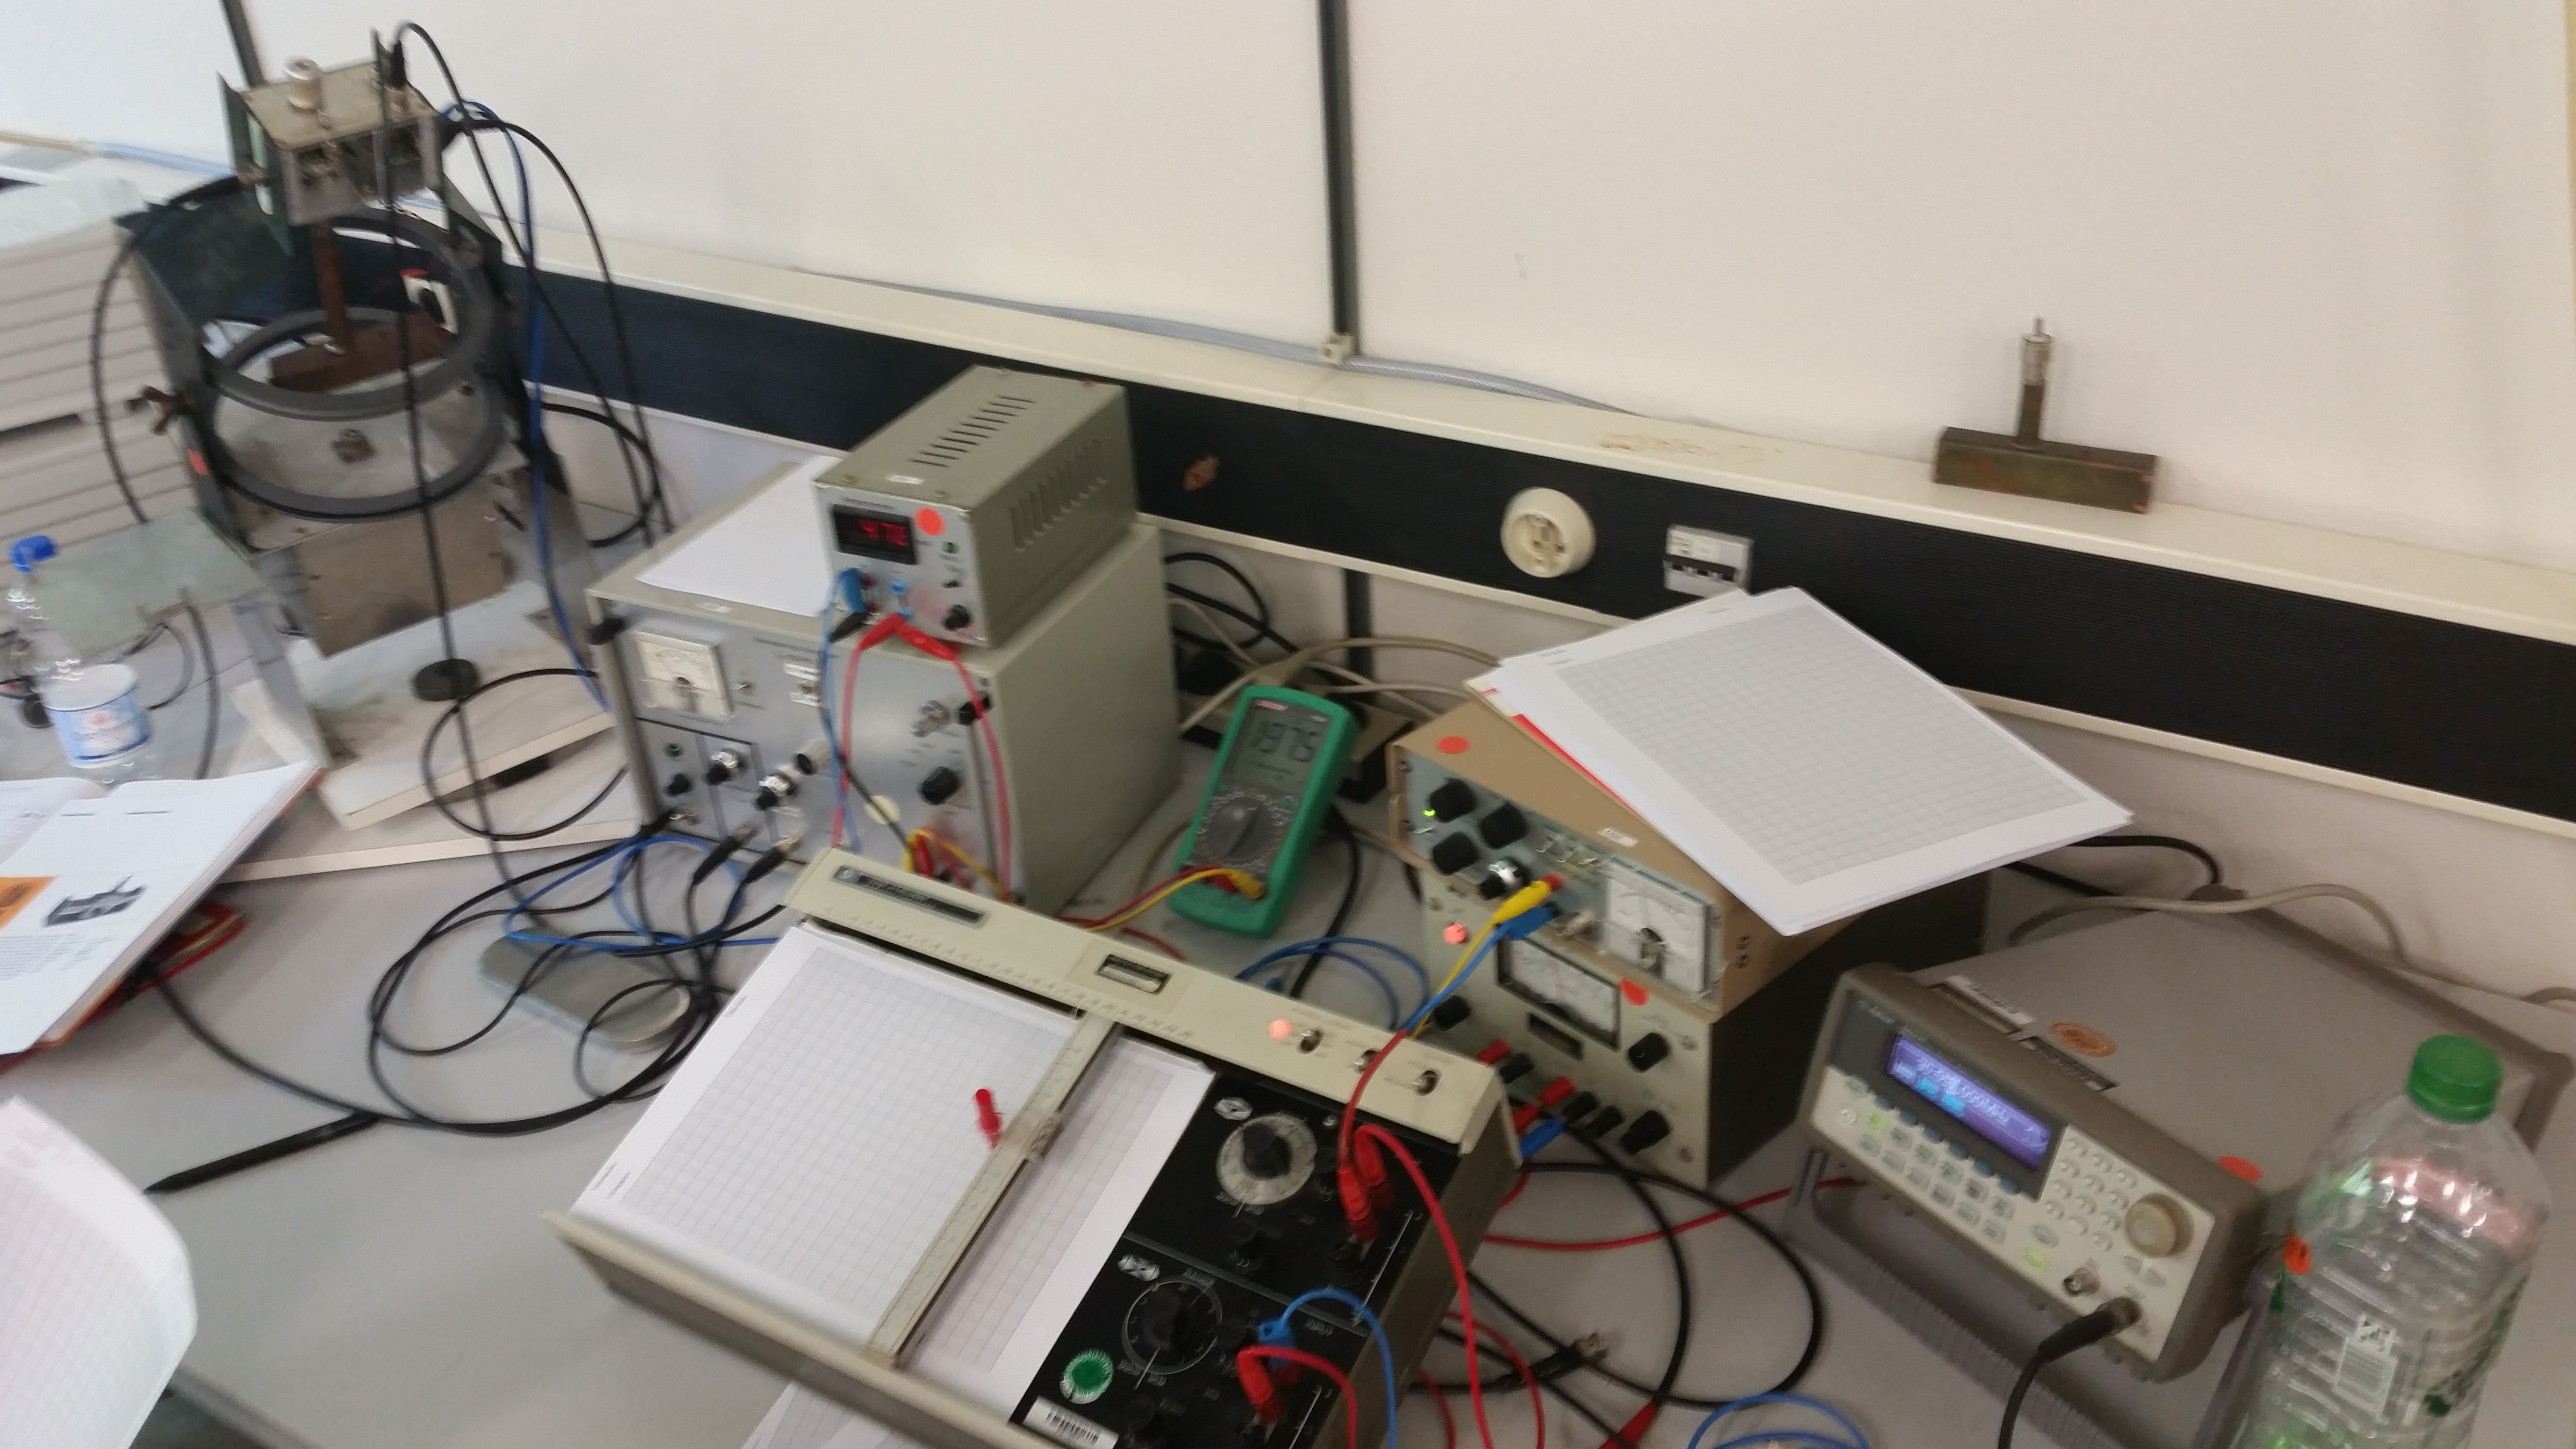
\includegraphics[width=\textwidth]{../Grafiken/Aufbau.jpg}};
			%\draw[step=.5cm,draw=gray] (0.0,0.0) grid (\textwidth,\textwidth - 180);
			%\foreach \x in {0,1,...,16}
			%	\filldraw [fill=green] (\x,0) node[below] {\x};
			%\foreach \y in {0,1,...,10}
			%	\filldraw [fill=green] (0,\y) node[left] {\y};
				
			\draw [thick] (2.0,7) -- (1.0,8.5);
			\node [draw=black,shape=circle,fill=lightgray] (1.) at (1.0,8.5) {1};
			\draw [thick] (3.0,7.5) -- (4.0,7.5);
			\node [draw=black,shape=circle,fill=lightgray] (1.) at (4.0,7.5) {2};
			\draw [thick] (5.0,5.5) -- (5.0,6.5);
			\node [draw=black,shape=circle,fill=lightgray] (1.) at (5.0,6.5) {3};
			\draw [thick] (6.0,6.5) -- (6.0,7.5);
			\node [draw=black,shape=circle,fill=lightgray] (1.) at (6.0,7.5) {4};
			\draw [thick] (8.0,4.5) -- (8.0,5.5);
			\node [draw=black,shape=circle,fill=lightgray] (1.) at (8.0,5.5) {5};
			\draw [thick] (7.0,3.0) -- (7.0,4.0);
			\node [draw=black,shape=circle,fill=lightgray] (1.) at (7.0,4.0) {6};
			\draw [thick] (9.5,4.5) -- (9.5,5.5);
			\node [draw=black,shape=circle,fill=lightgray] (1.) at (9.5,5.5) {7};
			\draw [thick] (10.5,2.) -- (10.5,1.);
			\node [draw=black,shape=circle,fill=lightgray] (1.) at (10.5,1.) {8};
			\draw [thick] (13,2.5) -- (13.,3.5);
			\node [draw=black,shape=circle,fill=lightgray] (1.) at (13.,3.5) {9};						

		\end{tikzpicture}
			\caption{Der verwendete Versuchsaufbau zur Durchführung von ESR-Messung}\label{fig:Aufbau}
\end{figure}
